\documentclass[times, utf8, seminar]{fer}
\usepackage{booktabs}
\usepackage{graphicx}
\usepackage{csquotes}
\graphicspath{{slike/}}

\begin{document}

\title{Preporučiteljski sustav Pixie}

\author{Petar Šegina}

\voditelj{Klemo Vladimir}

\maketitle

\tableofcontents

\chapter{Uvod}

Preporučiteljski sustav je sustav čija je zadaća predvidjeti korisnikov odabir nekog izbora\footnote{\cite{mmd}}. Takvi sustavi čine veoma važnu značajku modernih mrežnih usluga, nudeći korisnicima zanimljiv, bitan i njima personaliziran sadržaj. Time također mogu i povećati interakciju korisnika sa sadržajem za kojeg potencijalno nije ni svjestan da postoji, a koji bi mu mogao biti od interesa. Tako jedan glazbeni web dućan može povećati prodaju preporučivanjem pjesama i albuma sličnima onima za koje je korisnik pokazao interes, dok jedan portal s vijestima može korisniku preporučiti slične i zanimljive vijesti kako bi ga duže zadržao na samom portalu i povećao prihod od prikaza reklama.

Pinterest\footnote{\url{https://pinterest.com}} je moderna web usluga koja svojim korisnicima omogućuje otkrivanje novih i relevantnih ideja za izradu kreativnih projekata -- od kuharskih recepata pa do dizajna interijera. Riječima njihovog inženjerskog tima:

\begin{displayquote}
		  At Pinterest, a primary engineering challenge is helping people discover and do things every day, which means serving the right idea to the right person at the right time.\footnote{\cite{medium-article}}
\end{displayquote}

Pinterest je u svojoj srži preporučiteljski sustav te je važno da kao takav može dati korisne preporuke u dovoljno kratkom vremenu kako bi svojim korisnicima ponudio što veću vrijednost. Zbog veličine podataka i vremenskih zahtjeva kojima Pinterest barata, a koje ćemo iznijeti u nastavku, postojeća rješenja pokazivala su značajne nedostatke te je Pinterest za svoje potrebe odlučio napraviti vlastiti preporučiteljski sustav, naziva Pixie, koji se pokazao izrazito učinkovitim. Nad njihovim skupom podataka -- bipartitnog grafa od 3 milijarde čvorova povezanih sa 17 milijardi bridova, jedan Pixie poslužitelj može poslužiti 1.200 zahtjeva po sekundi sa latencijom u 99-om centilu unutar 60 milisekundi. S poslovne strane se Pixie također pokazao kao uspjeh jer je povećao i relevantnost preporuka koje se korisnicima nude i time povećao angažman korisnika za do 50\%\footnote{\cite{DBLP:journals/corr/abs-1711-07601}}.

U nastavku dajemo pregled preporučiteljskog sustava Pixie -- problema kojeg on pokušava riješiti, predloženo rješenje, primjer ostvarenja te rezultate koje to ostvarenje daje. Također nudimo i opis vlastite implementacije osnovnih algoritama preporučiteljskog sustava u programskom jeziku Kotlin\footnote{\url{https://kotlinlang.org}} te pregled dobivenih rezultata navedenog rješenja nad simuliranim skupom podataka.

\chapter{Problem}

\section{Generalizirani model}
Opišimo prvo općeniti problem preporučivanja koji pokušavamo riješiti. Model kojeg iznosimo ovdje inspiriran je formalnim modelom iznesenim u \cite{avsp-recommender}.

Krenimo od sustava koji se sastoji od dva skupa -- skupa korisnika \textit{K} i skupa predmeta \textit{P} s kojima korisnik može međudjelovati. Dodatno, svaki korisnik može za neki predmet iskazati koliko mu je taj predmet zanimljiv, što možemo modelirati funkcijom zanimljivosti $z = K \times P \to \mathbb{R}$ koja za danog korisnika i dani predmet vraća koliko je tom korisniku taj predmet zanimljiv.

Ukoliko za danog korisnika sortiramo skup predmeta po funkciji zanimljivosti, dobivamo listu predmeta poredanih po zanimljivosti za tog korisnika $P_k = sorted(P, z_k)$. Temeljem ove liste korisniku možemo preporučiti novi sadržaj uzimajući, primjerice, prvih 5 elemenata te liste.

Ovakav jednostavan model pokazuje temeljni zahtjev od preporučiteljskog sustava -- da na temelju poznatih informacija o korisniku može za njega preporučiti relevantan sadržaj. 

No, postoje određeni izazovi kojih je važno biti svjestan. Prvo je nepoznavanje funkcije z -- korisnik će eksplicitno izraziti zanimljivost tek za veoma maleni podskup predmeta. Kako bi mogli ponuditi preporuke, morati ćemo zanimljivost za ostale predmete procijeniti. Drugi bitan izazov je veličina skupa podataka -- $K \times P$ može biti velikih dimenzija, reda veličine $10^6 \times 10^6$ pa nećemo moći naivno obraditi cijeli skup podataka, već će biti nužno usredotočiti se na tek maleni podskup istih.

Postoje razni pristupi rješavanju ovog problema, od čega su možda najpopularniji preporučivanje temeljeno na sadržaju te suradničko filtriranje, koji su također dostupni kao gotovi algoritmi u programskom okviru \textit{Apache Mahout}\footnote{\cite{rovkp-mahout}}.

\section{Pinterestov problem}

Pogledajmo sada problem preporučivanja kojeg Pinterest pokušava riješiti. Vidjet ćemo da se određena svojstva specifična njihovom problemu mogu iskoristiti za bolje i efikasnije generiranje preporuka.

\subsection{Problem preporučivanja}

U Pinterestovom skupu podataka postoje dva tipa entiteta - pin (\textit{pribadača, značka} i board (\textit{ploča}). Svaki pin može biti povezan s više boardova i svaki board može imati više pinova, tj.\ relacija među njima je oblika N-N.

Te podatke možemo prikazati grafom na način da čvorove predstavljaju pinovi i boardovi, a bridove veze među njima. Kako ne postoji veza pin-pin niti veza board-board, navedeni graf je bipartitan. Kako su veze također dvosmjerne, graf je i neusmjeren.

\begin{figure}[h]
	\centering
	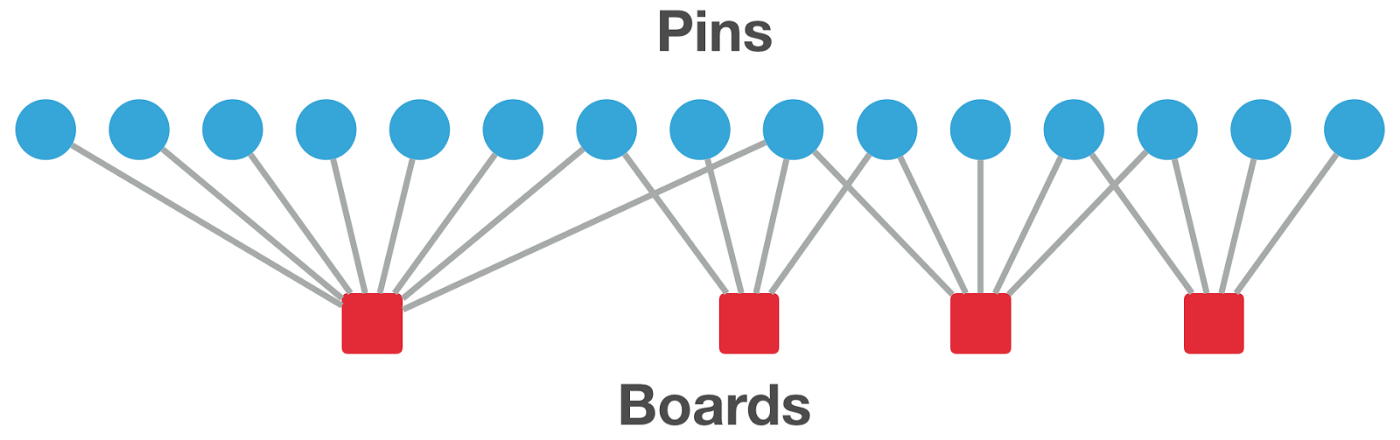
\includegraphics[width=\textwidth]{pins_boards_graph}
	\caption{Graf podataka}
	\cite{medium-article}
	\label{fig:pins_boards}
\end{figure}

Kada korisnik posjeti pin ili board, želja nam je pokušati preporučiti relevantne pinove kako bi korisnik mogao nastaviti svoju potragu u svome smjeru. Tako od preporučiteljskog sustava želimo da nam za dani pin i dani graf nađe druge pinove koji će korisniku biti zanimljivi.

Dodatno, ne želimo preporuku stvoriti samo na temelju jednog pina, već više njih koje je korisnik posjetio, s time da veći naglasak želimo staviti na one pinove koje je korisnik posjetio nedavno. Konačno, kako bi još više poboljšali preporuke, veći naglasak želimo staviti na one pinove koji bi korisniku mogli biti zanimljivi po nekim drugim parametrima koji nisu očiti iz grafa -- kao što su jezik sadržaja ili tema oko koje je sadržaj grupiran.

\subsection{Razmjer podataka i vremenski zahtjevi}

Važno je također posebnu pažnju skrenuti i na razmjer podataka kojima Pinterest barata. U svome radu\footnote{\cite{DBLP:journals/corr/abs-1711-07601}} ističu kako njihov graf sadrži 7 milijardi čvorova i 100 milijardi bridova. U radu također ističu i broj korisnika koji nadmašuje 200 milijuna.

Također treba istaknuti i vremenske zahtjeve na preporučiteljski sustav -- Pinterestu je važno da se preporuke mogu generirati u stvarnom vremenu, kako korisnik koristi sustav. Zbog toga je važno da izračun preporuka bude brz te je već čekanje od jedne sekunde previše i znatno bi narušilo krajnje korisničko iskustvo.

S ovim svime na umu, vidimo jasnu motivaciju zašto napraviti vlastiti preporučiteljski sustav -- oblik i količina podataka te vremenski zahtjevi nisu prikladni za pristup poput suradničkog filtriranja čije je vrijeme osvježavanja znatno duže i čiji prostorni zahtjevi nisu prikladni za red veličine miljardi.

\chapter{Rješenje}

Kako bi riješili navedeni problem, u Pinterestu su primijenili nekoliko inovativnih tehnika koje iskorištavaju oblik podataka kako bi generirale brz i relevantan odgovor.

\section{Jednostavna nasumična šetnja}

Algoritam Pixie zasnovan je na jednostavnoj nasumičnoj šetnji po grafu $G = (P, B, E) $.

Za dani graf G i početni pin $p \in P$, algoritam vrši nasumičnu šetnju u slijedećim koracima:

\begin{enumerate}
	\item Generiraj brojač $V: P \to \mathbb{N}$ s pretpostavljenom vrijednošću 0
	\item Za dani p nasumično odaberi $e_1 \in E$ koji povezuje p s nekim $b \in B$
	\item Za b nasumično odaberi $e_2 \in E$ koji povezuje b s nekim $p_2 \in P$
	\item Inkrementiraj $V[p_2]$
	\item Nastavi od koraka 2.\ koristeći $p_2$ kao početni pin
\end{enumerate}

Jasno je da ovaj algoritam neće nikad završiti pa zato ograničavamo duljinu šetnje na odabrani broj N. Nakon što algoritam završi, u brojaču V imamo broj posjećenosti svakog pina. Kako je vjerojatnije da će nasumična šetnja češće proći pinovima koji su početnom pinu bliski, broj pogodaka možemo koristiti kao mjeru sličnosti i kao preporuku vratiti one pinove koji su najčešće posjećeni.

Prednosti ovog algoritma su jednostavnost i performanse -- vrijeme izvođenja je konstantno u odnosu na veličinu grafa te ovisi samo o duljini šetnje, N.

No, za uspješan rad algoritma, potrebno je na ovu nasumičnu šetnju dodati još poneka poboljšanja.

\section{Dodavanje naklonosti nasumičnoj šetnji}

Primijetimo da prethodni algoritam ne uzima u obzir nikakva saznanja o korisniku. Za dva korisnika, $u_1$ i $u_2$, i isti početni pin $p$, preporuka će, ignoriravši nasumičnost šetnje, biti ista. Kako nam je želja dobiti preporuke koje će biti personalizirane za korisnika, potrebno je šetnju \textit{pogurnuti} u pravom smjeru. Prilika za to napraviti je prilikom odabira brida kojim će šetač proći. Umjesto nasumičnog odabira gdje svaki brid ima jednaku vjerojatnost da bude izabran, vjerojatnosti odabira se mogu izraziti kao pripadne težine bridova koje ovise o svojstvima trenutnog korisnika i predmeta koji se razmatra.

\section{Upiti sa više pinova i pripadnim težinama}

Kako bi se korisnika još bolje modeliralo, uz trenutni pin kojeg korisnik pregledava možemo uzeti u obzir i povijest pinova koje je korisnik pregledavao. Tako umjesto jednog upita q izvršimo skup upita Q i za svakog izračunamo pripadni brojač $V_q$.

Na kraju je potrebno dobivene brojače kombinirati. Brojače bi mogli kombinirati običnom sumom ili prosjekom, no nije svaki upit jednak. Naime, ako je početni pin jako povezan (ako se radi o čvoru visokog stupnja), biti će potrebno napraviti više koraka kako bi značajnost brojača bila jednaka onom dobivenom kretanjem od čvora niskog stupnja. U suprotnom bi preporuke generirane čvorovima niskog stupnja dominirale nad preporukama čvorova visokih stupanja, iako su potonji zbog svoje veće povezanosti u grafu značajniji.

Kako bi se riješio ovaj problem, za svaki upit q računa se faktor razmjera (\textit{scaling factor}) na slijedeći način:

\begin{centering}
		  $ k = |E(q)| $ \\
		  $ C = max_{p \in P}|E(p)| $ \\
		  $ s_q = k * (C - log(k)) $ \\
        k -- stupanj pin čvora upita \\
		  C -- najveći stupanj nekog pin čvora 
		  \par
\end{centering}

Na temelju tog faktora, računa se duljina šetnje pojedinog pina, $N_q$ temeljem ove formule:

\begin{centering}
	$ N_q = w_qN\frac{s_q}{\sigma_{r \in Q}s_r} $\par
\end{centering}

Distribucija duljine šetnji je sada takva da će šetnje koje počinju u čvorovima visokog stupnja imati razmjerno veću duljinu u odnosu na šetnje koje počinju u čvorovima niskog stupnja, ali će i dalje i ti čvorovi imati dovoljno duge šetnje.

Za potrebe ilustracije, generirali smo nasumičan skup od 40 čvorova stupnja između 1 i 100 i za svakog izračunali $N_q$ uz $N = 1000$ i $w_q = 1$. Vidljivo je da broj koraka raste linearno sa stupnjem čvora. Čvorovima stupnja 1 dodijeljena je šetnja duljine 45 koraka, a čvorovima stupnja 99 šetnja duljine 4328. Korišteni skup podataka dostupan je u popratnoj datoteci \textit{degree\_length\_chart.ods}.

\begin{figure}[h]
	\centering
	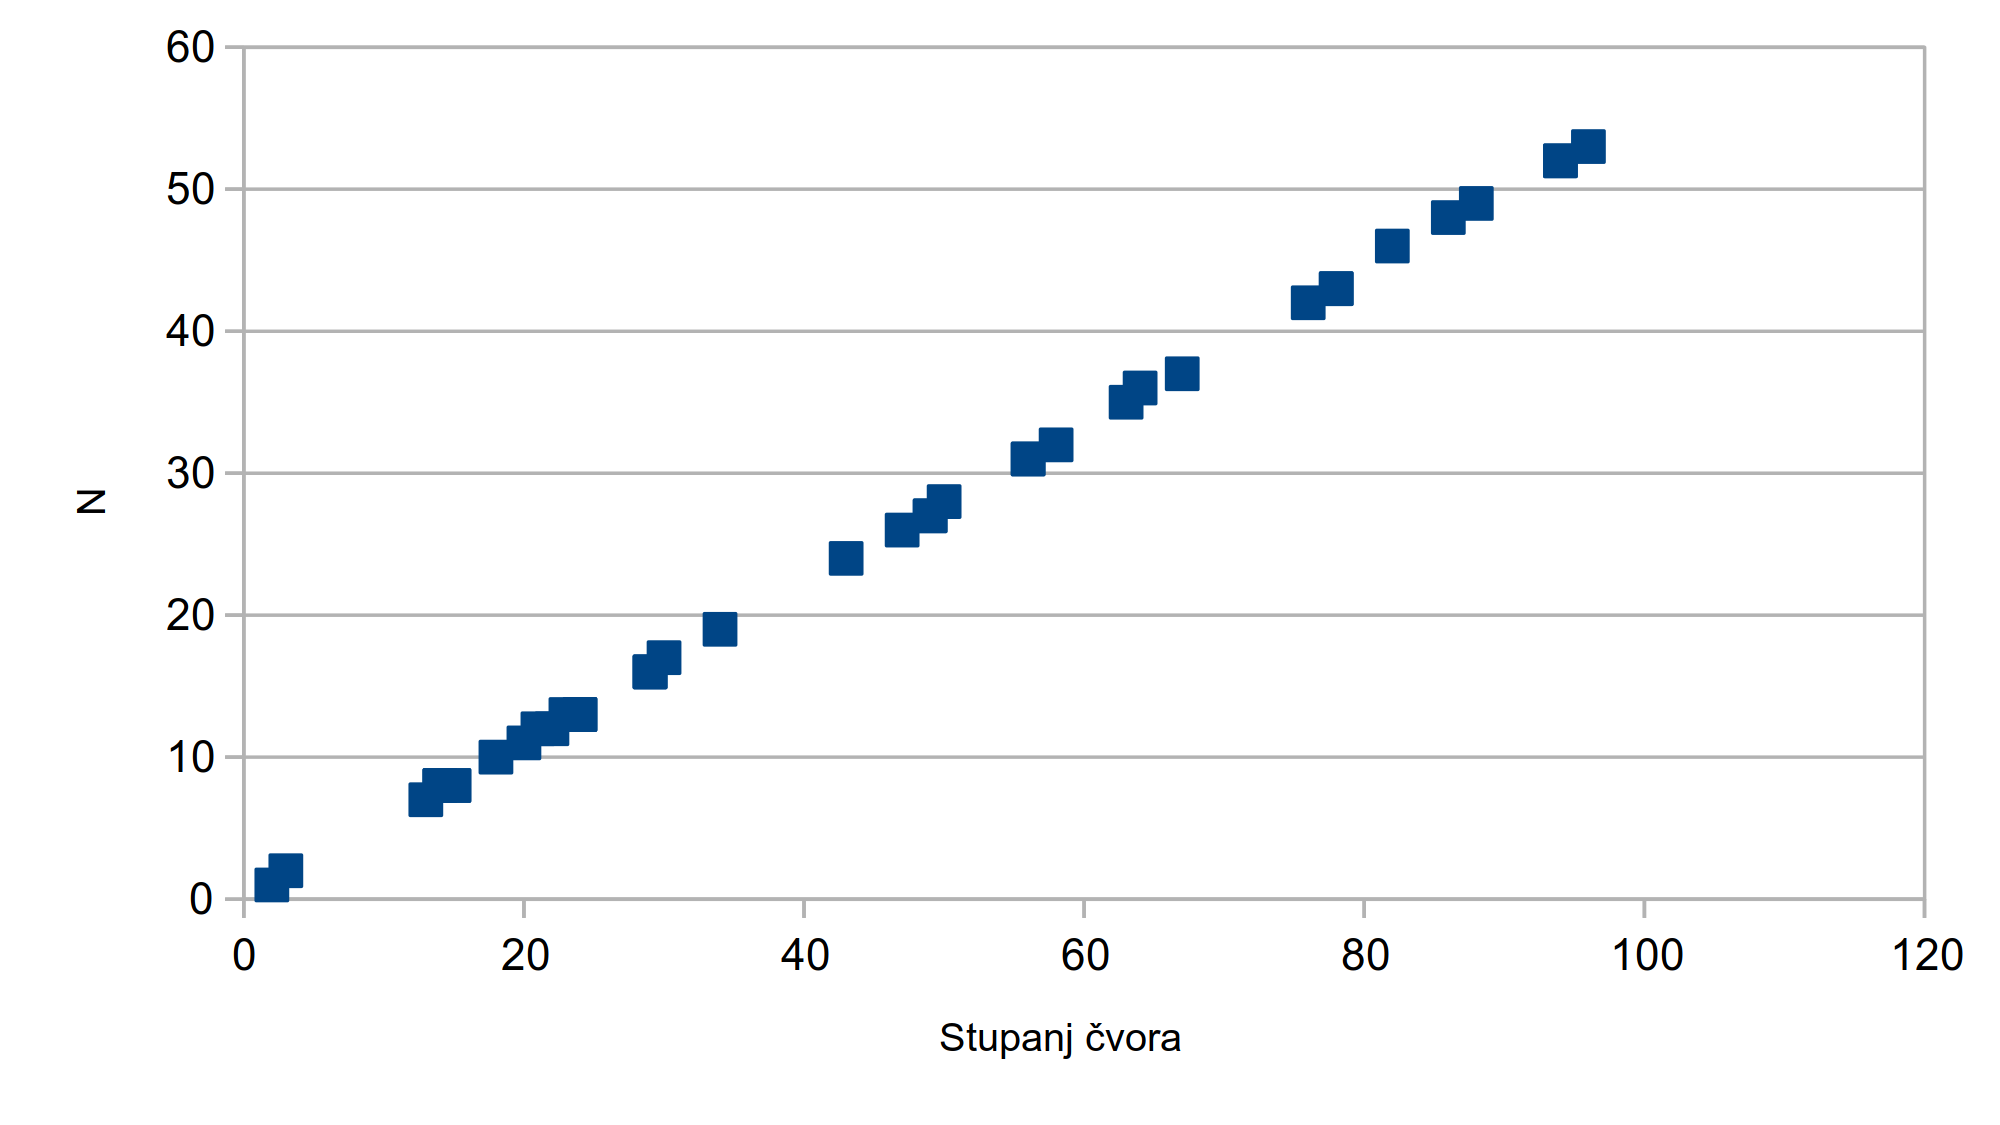
\includegraphics[width=\textwidth]{degree_chart}
	\caption{Odnos $k_q$ i $N_q$ za nasumično generiran skup podataka}
	\cite{medium-article}
	\label{fig:pins_boards}
\end{figure}

\section{Poticanje pinova koji se pojavljuju više puta}

\section{Rano zaustavljanje}

\section{Smanjivanje grafa}

\chapter{Ostvarenje}

\chapter{Rezultat}

\chapter{Zaključak}

\bibliography{literatura}
\bibliographystyle{fer}

\end{document}
